\section{Results}
\label{sec:results}

The thrust baseline result is obtained from the 1994 workflow with Iterative Bayesian
Unfolding at nominal $N_{\mathrm{iter}}=5$, including the hadronic event correction and
all configured systematic reruns.
All 14 nominal and systematic unfolding jobs completed successfully.
The response matrix diagonal fraction is 0.332, indicating substantial migration between
reconstructed and generated thrust bins; the maximum off-diagonal total correlation is
$|\rho_{ij}|=0.889$, confirming that correlated information is retained in the exported
products for downstream phenomenology.
In the central range ($0.60\le T<0.95$), the maximum total per-bin fractional uncertainty
is $42.1\%$, with individual components dominated by theory (max $32.9\%$) and
experimental (max $25.9\%$) variations; the endpoint bin ($0.99<T<1.00$) reaches a
ratio of $1.30\pm0.28$ relative to the published ALEPH 2004 result.

Table~\ref{tab:uncertainty_breakdown} summarizes the maximum per-bin fractional uncertainty
by component; Figs.~\ref{fig:per_bin_uncertainty}--\ref{fig:per_bin_uncertainty_theory}
and Tables~\ref{tab:per_bin_uncertainty}--\ref{tab:per_bin_uncertainty_breakdown_comparison} show
the full per-bin breakdown across the measurement range ($0.55\le T<1.0$).
Table~\ref{tab:per_bin_uncertainty_aleph} compares central values and total uncertainties with the
published ALEPH 2004 result; Table~\ref{tab:per_bin_uncertainty_breakdown_comparison} gives a
side-by-side component-level comparison (statistical, experimental/Sys.\,1, theory/Sys.\,2).

\begin{table}[t!]
\centering
\begin{tabular}{l c c}
\hline
Component & Max ($0.60\le T<0.95$) & Max ($0.50\le T<1.00$) \\
\hline
Statistical          & 13.1\% & 88.8\% \\
Unfolding iteration  &  0.86\% & 6.86\% \\
Experimental (total) & 25.9\% & 467.8\% \\
\quad track/event    & 24.4\% & 467.8\% \\
\quad neutral        & 12.4\% & 24.0\% \\
Theory               & 32.9\% & 343.2\% \\
Hadronic correction  & 25.5\% & 139.7\% \\
\hline
\textbf{Total}       & \textbf{42.1\%} & \textbf{500.9\%} \\
\hline
\end{tabular}
\caption{Maximum per-bin absolute fractional uncertainty by component for the thrust preliminary result. Full-range maxima are dominated by low-statistics endpoint bins; the central range ($0.60\le T < 0.95$) is the recommended reporting window. The experimental sub-rows (track/event, neutral) add in quadrature to form the experimental total.}
\label{tab:uncertainty_breakdown}
\end{table}


\begin{figure}[t!]
\centering
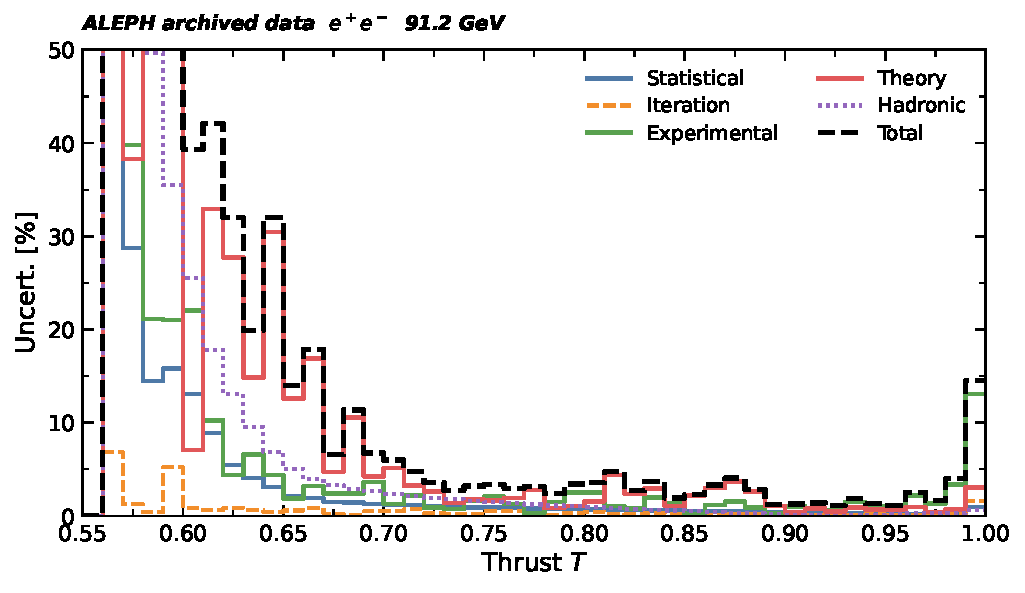
\includegraphics[width=0.72\textwidth]{../Studies/Phase2_Checks_2026-03-03/plots/uncertainty_breakdown/per_bin_uncertainty_grouped.pdf}
\caption{Per-bin absolute fractional uncertainty by group across the full measurement
range ($0.55\le T<1.0$): statistical, iteration envelope, experimental envelope,
theory envelope, hadronic correction, and total (dashed black). The $y$-axis is
limited to $50\%$.}
\label{fig:per_bin_uncertainty}
\end{figure}

\begin{figure}[t!]
\centering
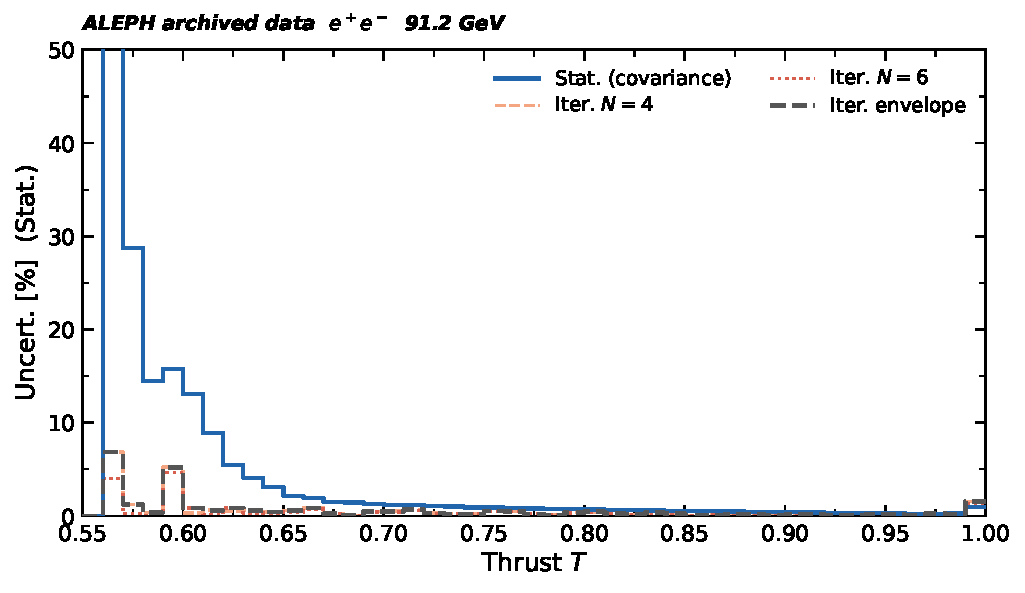
\includegraphics[width=0.72\textwidth]{../Studies/Phase2_Checks_2026-03-03/plots/uncertainty_breakdown/per_bin_uncertainty_stat.pdf}
\caption{Statistical and iteration-uncertainty breakdown. Dashed/dotted lines show
the signed variation for $N_{\mathrm{iter}}=4$ and $6$; the dashed-black line is the
iteration envelope. The $y$-axis is limited to $50\%$.}
\label{fig:per_bin_uncertainty_stat}
\end{figure}

\begin{figure}[t!]
\centering
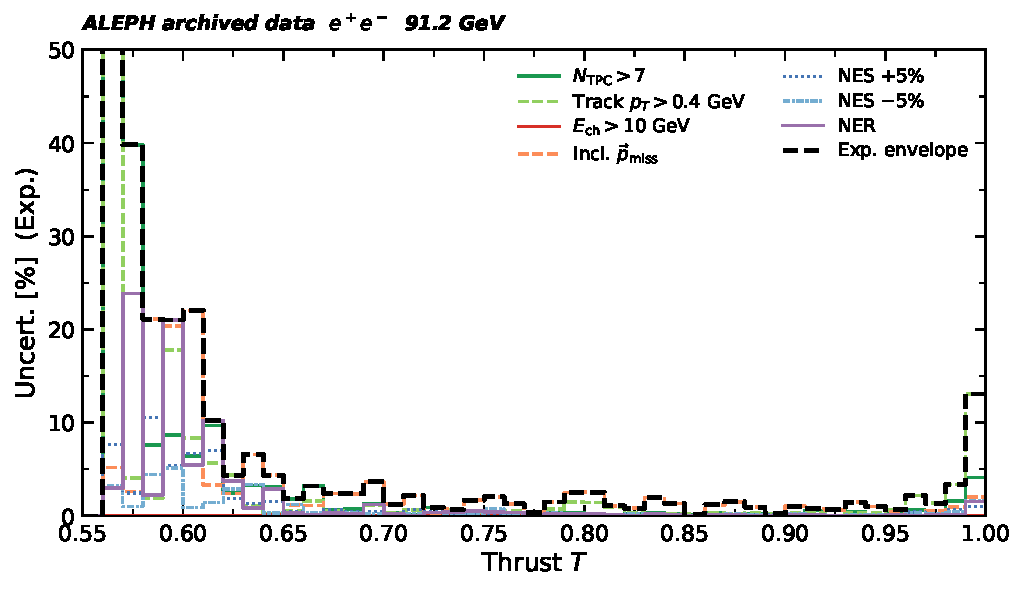
\includegraphics[width=0.72\textwidth]{../Studies/Phase2_Checks_2026-03-03/plots/uncertainty_breakdown/per_bin_uncertainty_exp.pdf}
\caption{Experimental uncertainty breakdown: seven individual variation branches
(track/event and neutral) with the group envelope (dashed black).
Large values at $T\lesssim 0.62$ arise because the nominal spectrum is steeply
rising from near zero there; even small absolute shifts produce large fractional
changes. The $y$-axis is limited to $50\%$.}
\label{fig:per_bin_uncertainty_exp}
\end{figure}

\begin{figure}[t!]
\centering
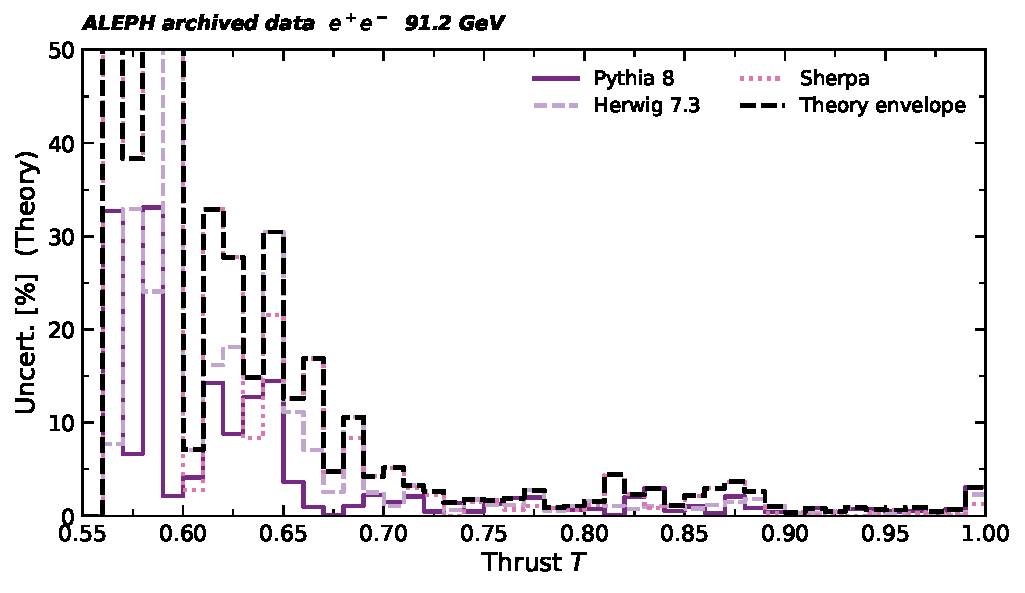
\includegraphics[width=0.72\textwidth]{../Studies/Phase2_Checks_2026-03-03/plots/uncertainty_breakdown/per_bin_uncertainty_theory.pdf}
\caption{Theory uncertainty breakdown: Pythia~8, Herwig~7.3, and Sherpa individual
shifts with the theory envelope (dashed black). The $y$-axis is limited to $50\%$.}
\label{fig:per_bin_uncertainty_theory}
\end{figure}

\begin{table}[t!]
\centering
\scriptsize
\begin{tabular}{c r c c c c c c}
\hline
$T$ range & $(1/\sigma)\,\mathrm{d}\sigma/\mathrm{d}T$ & Stat. & Iter. & Exp. & Theory & Had.\ corr. & Total \\
 & & [\%] & [\%] & [\%] & [\%] & [\%] & [\%] \\
\hline
[0.55,0.56) & \multicolumn{7}{c}{---} \\
{[0.56,0.57)} & $6.30\times10^{-5}$ & 88.8 & 6.9 & 467.8 & 67.7 & 139.7 & 500.9 \\
{[0.57,0.58)} & 0.0012 & 28.8 & 1.2 & 46.7 & 38.3 & 70.5 & 97.2 \\
{[0.58,0.59)} & 0.0015 & 14.5 & 0.4 & 25.0 & 59.5 & 49.6 & 82.7 \\
{[0.59,0.60)} & 0.0032 & 15.8 & 5.2 & 35.8 & 53.5 & 35.5 & 75.3 \\
{[0.60,0.61)} & 0.0042 & 13.1 & 0.9 & 25.9 & 7.1 & 25.5 & 39.3 \\
{[0.61,0.62)} & 0.0085 & 8.9 & 0.6 & 17.1 & 32.9 & 17.8 & 42.1 \\
{[0.62,0.63)} & 0.0131 & 5.5 & 0.9 & 7.3 & 27.7 & 13.0 & 32.0 \\
{[0.63,0.64)} & 0.0248 & 4.1 & 0.6 & 8.2 & 14.8 & 9.6 & 19.9 \\
{[0.64,0.65)} & 0.0411 & 3.1 & 0.5 & 6.3 & 30.5 & 6.9 & 32.0 \\
{[0.65,0.66)} & 0.0695 & 2.2 & 0.6 & 2.6 & 12.6 & 5.0 & 14.0 \\
{[0.66,0.67)} & 0.1068 & 1.9 & 0.8 & 3.8 & 16.9 & 3.9 & 17.9 \\
{[0.67,0.68)} & 0.1305 & 1.5 & 0.3 & 2.7 & 4.7 & 3.4 & 6.6 \\
{[0.68,0.69)} & 0.1587 & 1.5 & 0.1 & 2.6 & 10.6 & 2.9 & 11.4 \\
{[0.69,0.70)} & 0.1776 & 1.3 & 0.5 & 4.3 & 4.3 & 2.7 & 6.7 \\
{[0.70,0.71)} & 0.2087 & 1.2 & 0.5 & 1.4 & 5.2 & 2.4 & 6.0 \\
{[0.71,0.72)} & 0.2448 & 1.2 & 0.7 & 2.4 & 3.3 & 2.1 & 4.8 \\
{[0.72,0.73)} & 0.2876 & 1.0 & 0.3 & 1.1 & 2.6 & 1.9 & 3.6 \\
{[0.73,0.74)} & 0.3210 & 1.0 & 0.2 & 1.2 & 1.4 & 1.8 & 2.8 \\
{[0.74,0.75)} & 0.3792 & 0.9 & 0.2 & 1.9 & 1.8 & 1.6 & 3.2 \\
{[0.75,0.76)} & 0.4332 & 0.9 & 0.6 & 2.3 & 1.7 & 1.5 & 3.4 \\
{[0.76,0.77)} & 0.4958 & 0.8 & 0.5 & 1.5 & 1.9 & 1.4 & 3.0 \\
{[0.77,0.78)} & 0.5504 & 0.8 & 0.2 & 0.5 & 2.8 & 1.2 & 3.2 \\
{[0.78,0.79)} & 0.5994 & 0.7 & 0.1 & 1.8 & 0.9 & 1.1 & 2.4 \\
{[0.79,0.80)} & 0.6550 & 0.8 & 0.4 & 3.0 & 1.1 & 1.0 & 3.4 \\
{[0.80,0.81)} & 0.7399 & 0.7 & 0.5 & 3.0 & 1.6 & 0.9 & 3.6 \\
{[0.81,0.82)} & 0.8395 & 0.7 & 0.3 & 1.4 & 4.4 & 0.8 & 4.8 \\
{[0.82,0.83)} & 0.9697 & 0.6 & 0.2 & 0.9 & 2.3 & 0.8 & 2.7 \\
{[0.83,0.84)} & 1.14 & 0.6 & 0.3 & 2.0 & 3.0 & 0.7 & 3.7 \\
{[0.84,0.85)} & 1.26 & 0.6 & 0.3 & 1.4 & 1.1 & 0.6 & 1.9 \\
{[0.85,0.86)} & 1.45 & 0.5 & 0.0 & 0.3 & 2.2 & 0.5 & 2.3 \\
{[0.86,0.87)} & 1.64 & 0.5 & 0.1 & 1.3 & 3.0 & 0.4 & 3.3 \\
{[0.87,0.88)} & 1.89 & 0.5 & 0.2 & 1.6 & 3.7 & 0.4 & 4.1 \\
{[0.88,0.89)} & 2.23 & 0.5 & 0.2 & 1.0 & 2.6 & 0.3 & 2.9 \\
{[0.89,0.90)} & 2.67 & 0.4 & 0.1 & 0.4 & 1.0 & 0.2 & 1.2 \\
{[0.90,0.91)} & 3.20 & 0.4 & 0.1 & 1.2 & 0.4 & 0.1 & 1.3 \\
{[0.91,0.92)} & 3.86 & 0.4 & 0.2 & 1.1 & 0.8 & 0.1 & 1.4 \\
{[0.92,0.93)} & 4.70 & 0.4 & 0.1 & 0.9 & 0.5 & 0.0 & 1.1 \\
{[0.93,0.94)} & 5.79 & 0.3 & 0.1 & 1.6 & 0.9 & 0.1 & 1.9 \\
{[0.94,0.95)} & 7.40 & 0.3 & 0.2 & 1.1 & 0.7 & 0.1 & 1.4 \\
{[0.95,0.96)} & 9.79 & 0.3 & 0.1 & 0.8 & 0.6 & 0.2 & 1.1 \\
{[0.96,0.97)} & 13.86 & 0.2 & 0.1 & 2.3 & 1.0 & 0.3 & 2.5 \\
{[0.97,0.98)} & 18.46 & 0.2 & 0.3 & 1.5 & 0.5 & 0.4 & 1.6 \\
{[0.98,0.99)} & 12.18 & 0.3 & 0.2 & 3.9 & 0.7 & 0.3 & 4.0 \\
{[0.99,1.00)} & 1.01 & 1.0 & 1.6 & 14.1 & 3.1 & 0.7 & 14.5 \\
\hline
\end{tabular}
\normalsize
\caption{Per-bin fractional uncertainties across the full measurement range ($0.55 \leq T < 1.0$). The second column gives the nominal unfolded $(1/\sigma)\,\mathrm{d}\sigma/\mathrm{d}T$ value; all remaining columns are absolute fractional uncertainties in percent. Bins with zero nominal spectrum (dashes) are below threshold. \textit{Exp.} denotes the total experimental component (track/event and neutral sub-components combined in quadrature), and \textit{Had.\ corr.} denotes the hadronic event-selection correction uncertainty.}
\label{tab:per_bin_uncertainty}
\end{table}

\begin{table}[t!]
\centering
\scriptsize
\begin{tabular}{c r r r r}
\hline
$T$ range & Our $(1/\sigma)\,\mathrm{d}\sigma/\mathrm{d}T$ & Our total unc.\ [\%] & ALEPH 2004 $(1/\sigma)\,\mathrm{d}\sigma/\mathrm{d}T$ & ALEPH 2004 total unc.\ [\%] \\
\hline
[0.55,0.56) & \multicolumn{1}{c}{---} & \multicolumn{1}{c}{---} & \multicolumn{1}{c}{---} & \multicolumn{1}{c}{---} \\
{[0.56,0.57)} & $6.30\times10^{-5}$ & 500.9 & \multicolumn{1}{c}{---} & \multicolumn{1}{c}{---} \\
{[0.57,0.58)} & 0.0012 & 97.2 & \multicolumn{1}{c}{---} & \multicolumn{1}{c}{---} \\
{[0.58,0.59)} & 0.0015 & 82.7 & 0.0011 & 61.2 \\
{[0.59,0.60)} & 0.0032 & 75.3 & 0.0023 & 54.1 \\
{[0.60,0.61)} & 0.0042 & 39.3 & 0.0035 & 41.7 \\
{[0.61,0.62)} & 0.0085 & 42.1 & 0.0084 & 25.0 \\
{[0.62,0.63)} & 0.0131 & 32.0 & 0.0128 & 23.1 \\
{[0.63,0.64)} & 0.0248 & 19.9 & 0.0215 & 21.9 \\
{[0.64,0.65)} & 0.0411 & 32.0 & 0.0433 & 14.4 \\
{[0.65,0.66)} & 0.0695 & 14.0 & 0.0656 & 9.2 \\
{[0.66,0.67)} & 0.1068 & 17.9 & 0.1028 & 8.5 \\
{[0.67,0.68)} & 0.1305 & 6.6 & 0.1258 & 8.7 \\
{[0.68,0.69)} & 0.1587 & 11.4 & 0.1640 & 8.7 \\
{[0.69,0.70)} & 0.1776 & 6.7 & 0.1842 & 9.5 \\
{[0.70,0.71)} & 0.2087 & 6.0 & 0.2142 & 7.6 \\
{[0.71,0.72)} & 0.2448 & 4.8 & 0.2481 & 9.1 \\
{[0.72,0.73)} & 0.2876 & 3.6 & 0.2943 & 7.5 \\
{[0.73,0.74)} & 0.3210 & 2.8 & 0.3435 & 6.2 \\
{[0.74,0.75)} & 0.3792 & 3.2 & 0.3654 & 6.0 \\
{[0.75,0.76)} & 0.4332 & 3.4 & 0.4309 & 6.0 \\
{[0.76,0.77)} & 0.4958 & 3.0 & 0.4692 & 4.9 \\
{[0.77,0.78)} & 0.5504 & 3.2 & 0.5458 & 4.2 \\
{[0.78,0.79)} & 0.5994 & 2.4 & 0.5994 & 4.2 \\
{[0.79,0.80)} & 0.6550 & 3.4 & 0.6609 & 5.6 \\
{[0.80,0.81)} & 0.7399 & 3.6 & 0.7680 & 4.6 \\
{[0.81,0.82)} & 0.8395 & 4.8 & 0.8570 & 4.3 \\
{[0.82,0.83)} & 0.9697 & 2.7 & 0.9808 & 5.1 \\
{[0.83,0.84)} & 1.14 & 3.7 & 1.11 & 5.0 \\
{[0.84,0.85)} & 1.26 & 1.9 & 1.27 & 4.9 \\
{[0.85,0.86)} & 1.45 & 2.3 & 1.44 & 3.8 \\
{[0.86,0.87)} & 1.64 & 3.3 & 1.64 & 4.0 \\
{[0.87,0.88)} & 1.89 & 4.1 & 1.93 & 3.9 \\
{[0.88,0.89)} & 2.23 & 2.9 & 2.23 & 3.4 \\
{[0.89,0.90)} & 2.67 & 1.2 & 2.63 & 3.2 \\
{[0.90,0.91)} & 3.20 & 1.3 & 3.06 & 3.3 \\
{[0.91,0.92)} & 3.86 & 1.4 & 3.70 & 2.2 \\
{[0.92,0.93)} & 4.70 & 1.1 & 4.55 & 2.3 \\
{[0.93,0.94)} & 5.79 & 1.9 & 5.64 & 2.2 \\
{[0.94,0.95)} & 7.40 & 1.4 & 7.28 & 1.7 \\
{[0.95,0.96)} & 9.79 & 1.1 & 9.63 & 1.7 \\
{[0.96,0.97)} & 13.86 & 2.5 & 13.60 & 1.7 \\
{[0.97,0.98)} & 18.46 & 1.6 & 18.57 & 3.7 \\
{[0.98,0.99)} & 12.18 & 4.0 & 12.89 & 4.1 \\
{[0.99,1.00)} & 1.01 & 14.5 & 1.31 & 15.4 \\
\hline
\end{tabular}
\normalsize
\caption{Comparison of the nominal unfolded $(1/\sigma)\,\mathrm{d}\sigma/\mathrm{d}T$ and total fractional uncertainty with the published ALEPH 2004 result (HEPData ins:636645, Table~54) across the full measurement range ($0.55\le T<1.0$). The ALEPH 2004 total uncertainty combines statistical, sys$_1$, and sys$_2$ components in quadrature. Dashes indicate bins not covered by one or both measurements.}
\label{tab:per_bin_uncertainty_aleph}
\end{table}

\begin{table}[t!]
\centering
\scriptsize
\resizebox{\textwidth}{!}{%
\begin{tabular}{c  r r r r  r r r r  r r}
\hline
& \multicolumn{2}{c}{$(1/\sigma)\,\mathrm{d}\sigma/\mathrm{d}T$}
 & \multicolumn{2}{c}{Stat.\ [\%]}
 & \multicolumn{2}{c}{Exp.\ / Sys.\,1 [\%]}
 & \multicolumn{2}{c}{Theory\,/ Sys.\,2 [\%]}
 & \multicolumn{2}{c}{Total [\%]} \\
\cline{2-3}\cline{4-5}\cline{6-7}\cline{8-9}\cline{10-11}
$T$ range & Ours & ALEPH & Ours & ALEPH & Ours & ALEPH & Ours & ALEPH & Ours & ALEPH \\
\hline
{[0.55,0.56)} & \multicolumn{10}{c}{---} \\
{[0.56,0.57)} & $6.30{\times}10^{-5}$ & --- & 88.8 & --- & 467.8 & --- & 67.7 & --- & 500.9 & --- \\
{[0.57,0.58)} & $1.22{\times}10^{-3}$ & --- & 28.8 & --- & 46.7 & --- & 38.3 & --- & 97.2 & --- \\
{[0.58,0.59)} & $1.48{\times}10^{-3}$ & $1.15{\times}10^{-3}$ & 14.5 & 29.6 & 25.0 & 45.2 & 59.5 & 28.7 & 82.7 & 61.2 \\
{[0.59,0.60)} & $3.23{\times}10^{-3}$ & $2.29{\times}10^{-3}$ & 15.8 & 21.8 & 35.8 & 40.6 & 53.5 & 28.4 & 75.3 & 54.1 \\
{[0.60,0.61)} & $4.20{\times}10^{-3}$ & $3.50{\times}10^{-3}$ & 13.1 & 17.4 & 25.9 & 24.9 & 7.1 & 28.6 & 39.3 & 41.7 \\
{[0.61,0.62)} & $8.53{\times}10^{-3}$ & $8.39{\times}10^{-3}$ & 8.9 & 11.4 & 17.1 & 9.2 & 32.9 & 20.3 & 42.1 & 25.0 \\
{[0.62,0.63)} & 0.0131 & 0.0128 & 5.5 & 9.0 & 7.3 & 6.4 & 27.7 & 20.3 & 32.0 & 23.1 \\
{[0.63,0.64)} & 0.0248 & 0.0215 & 4.1 & 7.1 & 8.2 & 4.4 & 14.8 & 20.3 & 19.9 & 21.9 \\
{[0.64,0.65)} & 0.0411 & 0.0433 & 3.1 & 5.2 & 6.3 & 11.5 & 30.5 & 7.1 & 32.0 & 14.4 \\
{[0.65,0.66)} & 0.0695 & 0.0656 & 2.2 & 4.1 & 2.6 & 4.2 & 12.6 & 7.1 & 14.0 & 9.2 \\
{[0.66,0.67)} & 0.1068 & 0.1028 & 1.9 & 3.2 & 3.8 & 3.4 & 16.9 & 7.1 & 17.9 & 8.5 \\
{[0.67,0.68)} & 0.1305 & 0.1258 & 1.5 & 2.9 & 2.7 & 2.4 & 4.7 & 7.8 & 6.6 & 8.7 \\
{[0.68,0.69)} & 0.1587 & 0.1640 & 1.5 & 2.5 & 2.6 & 2.9 & 10.6 & 7.8 & 11.4 & 8.7 \\
{[0.69,0.70)} & 0.1776 & 0.1842 & 1.3 & 2.4 & 4.3 & 4.7 & 4.3 & 7.8 & 6.7 & 9.5 \\
{[0.70,0.71)} & 0.2087 & 0.2142 & 1.2 & 2.2 & 1.4 & 2.1 & 5.2 & 7.0 & 6.0 & 7.6 \\
{[0.71,0.72)} & 0.2448 & 0.2481 & 1.2 & 2.1 & 2.4 & 5.4 & 3.3 & 7.0 & 4.8 & 9.1 \\
{[0.72,0.73)} & 0.2876 & 0.2943 & 1.0 & 1.9 & 1.1 & 1.9 & 2.6 & 7.0 & 3.6 & 7.5 \\
{[0.73,0.74)} & 0.3210 & 0.3435 & 1.0 & 1.8 & 1.2 & 2.3 & 1.4 & 5.5 & 2.8 & 6.2 \\
{[0.74,0.75)} & 0.3792 & 0.3654 & 0.9 & 1.7 & 1.9 & 1.9 & 1.8 & 5.5 & 3.2 & 6.0 \\
{[0.75,0.76)} & 0.4332 & 0.4309 & 0.9 & 1.6 & 2.3 & 2.0 & 1.7 & 5.5 & 3.4 & 6.0 \\
{[0.76,0.77)} & 0.4958 & 0.4692 & 0.8 & 1.5 & 1.5 & 2.8 & 1.9 & 3.7 & 3.0 & 4.9 \\
{[0.77,0.78)} & 0.5504 & 0.5458 & 0.8 & 1.4 & 0.5 & 1.3 & 2.8 & 3.7 & 3.2 & 4.2 \\
{[0.78,0.79)} & 0.5994 & 0.5994 & 0.7 & 1.4 & 1.8 & 1.3 & 0.9 & 3.7 & 2.4 & 4.2 \\
{[0.79,0.80)} & 0.6550 & 0.6609 & 0.8 & 1.3 & 3.0 & 3.7 & 1.1 & 3.9 & 3.4 & 5.6 \\
{[0.80,0.81)} & 0.7399 & 0.7680 & 0.7 & 1.2 & 3.0 & 2.0 & 1.6 & 3.9 & 3.6 & 4.6 \\
{[0.81,0.82)} & 0.8395 & 0.8570 & 0.7 & 1.1 & 1.4 & 1.4 & 4.4 & 3.9 & 4.8 & 4.3 \\
{[0.82,0.83)} & 0.9697 & 0.9808 & 0.6 & 1.1 & 0.9 & 1.3 & 2.3 & 4.8 & 2.7 & 5.1 \\
{[0.83,0.84)} & 1.14 & 1.11 & 0.6 & 1.0 & 2.0 & 0.8 & 3.0 & 4.8 & 3.7 & 5.0 \\
{[0.84,0.85)} & 1.26 & 1.27 & 0.6 & 1.0 & 1.4 & 0.7 & 1.1 & 4.8 & 1.9 & 4.9 \\
{[0.85,0.86)} & 1.45 & 1.44 & 0.5 & 0.9 & 0.3 & 0.7 & 2.2 & 3.6 & 2.3 & 3.8 \\
{[0.86,0.87)} & 1.64 & 1.64 & 0.5 & 0.8 & 1.3 & 1.5 & 3.0 & 3.6 & 3.3 & 4.0 \\
{[0.87,0.88)} & 1.89 & 1.93 & 0.5 & 0.8 & 1.6 & 1.3 & 3.7 & 3.6 & 4.1 & 3.9 \\
{[0.88,0.89)} & 2.23 & 2.23 & 0.5 & 0.7 & 1.0 & 1.3 & 2.6 & 3.1 & 2.9 & 3.4 \\
{[0.89,0.90)} & 2.67 & 2.63 & 0.4 & 0.7 & 0.4 & 0.6 & 1.0 & 3.1 & 1.2 & 3.2 \\
{[0.90,0.91)} & 3.20 & 3.06 & 0.4 & 0.6 & 1.2 & 1.1 & 0.4 & 3.1 & 1.3 & 3.3 \\
{[0.91,0.92)} & 3.86 & 3.70 & 0.4 & 0.6 & 1.1 & 0.6 & 0.8 & 2.1 & 1.4 & 2.2 \\
{[0.92,0.93)} & 4.70 & 4.55 & 0.4 & 0.5 & 0.9 & 0.8 & 0.5 & 2.1 & 1.1 & 2.3 \\
{[0.93,0.94)} & 5.79 & 5.64 & 0.3 & 0.5 & 1.6 & 0.7 & 0.9 & 2.1 & 1.9 & 2.2 \\
{[0.94,0.95)} & 7.40 & 7.28 & 0.3 & 0.4 & 1.1 & 0.6 & 0.7 & 1.5 & 1.4 & 1.7 \\
{[0.95,0.96)} & 9.79 & 9.63 & 0.3 & 0.4 & 0.8 & 0.7 & 0.6 & 1.5 & 1.1 & 1.7 \\
{[0.96,0.97)} & 13.9 & 13.6 & 0.2 & 0.3 & 2.3 & 0.6 & 1.0 & 1.5 & 2.5 & 1.7 \\
{[0.97,0.98)} & 18.5 & 18.6 & 0.2 & 0.3 & 1.5 & 0.5 & 0.5 & 3.7 & 1.6 & 3.7 \\
{[0.98,0.99)} & 12.2 & 12.9 & 0.3 & 0.3 & 3.9 & 1.8 & 0.7 & 3.7 & 4.0 & 4.1 \\
{[0.99,1.00)} & 1.01 & 1.31 & 1.0 & 0.8 & 14.1 & 14.9 & 3.1 & 3.7 & 14.5 & 15.4 \\
\hline
\end{tabular}
}% end resizebox
\normalsize
\caption{Per-bin fractional uncertainty breakdown comparison between this analysis and the published ALEPH 2004 result (HEPData ins:636645, Table~54). For this analysis, Stat.\ is derived from the RooUnfold covariance, Exp.\ is the quadrature sum of all experimental track/event and neutral variations, and Theory is the max envelope of the three generator reweightings. For ALEPH 2004, Sys.\,1 and Sys.\,2 correspond to the two systematic components provided in the HEPData table. All values are absolute fractional uncertainties in percent; Total combines all components in quadrature. Dashes indicate bins outside the respective measurement range.}
\label{tab:per_bin_uncertainty_breakdown_comparison}
\end{table}


\subsection{Uncertainty structure across components}

\begin{figure}[t!]
\centering
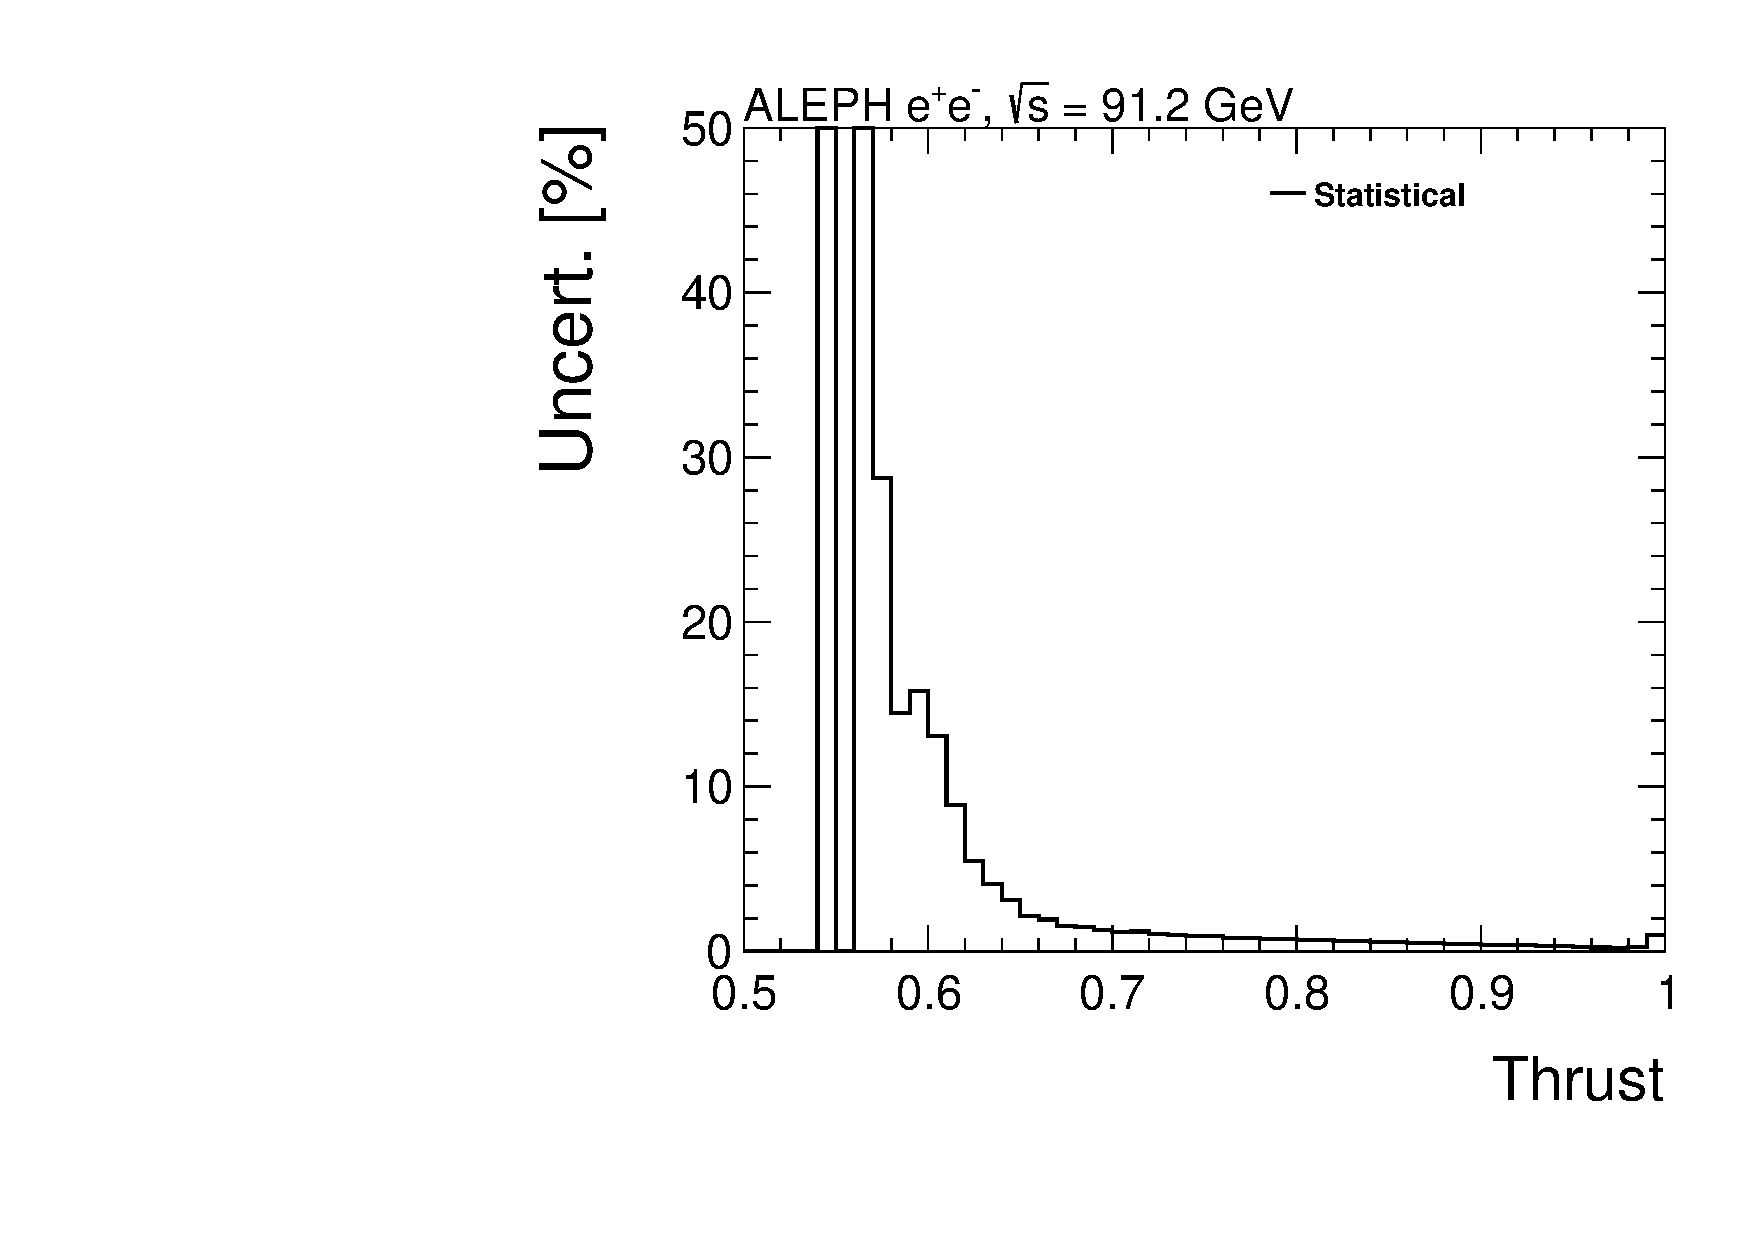
\includegraphics[width=0.49\textwidth]{../Studies/PreliminaryResult/2026-02-17_thrust_iter5/summary/uncertainty_components_statistical.pdf}
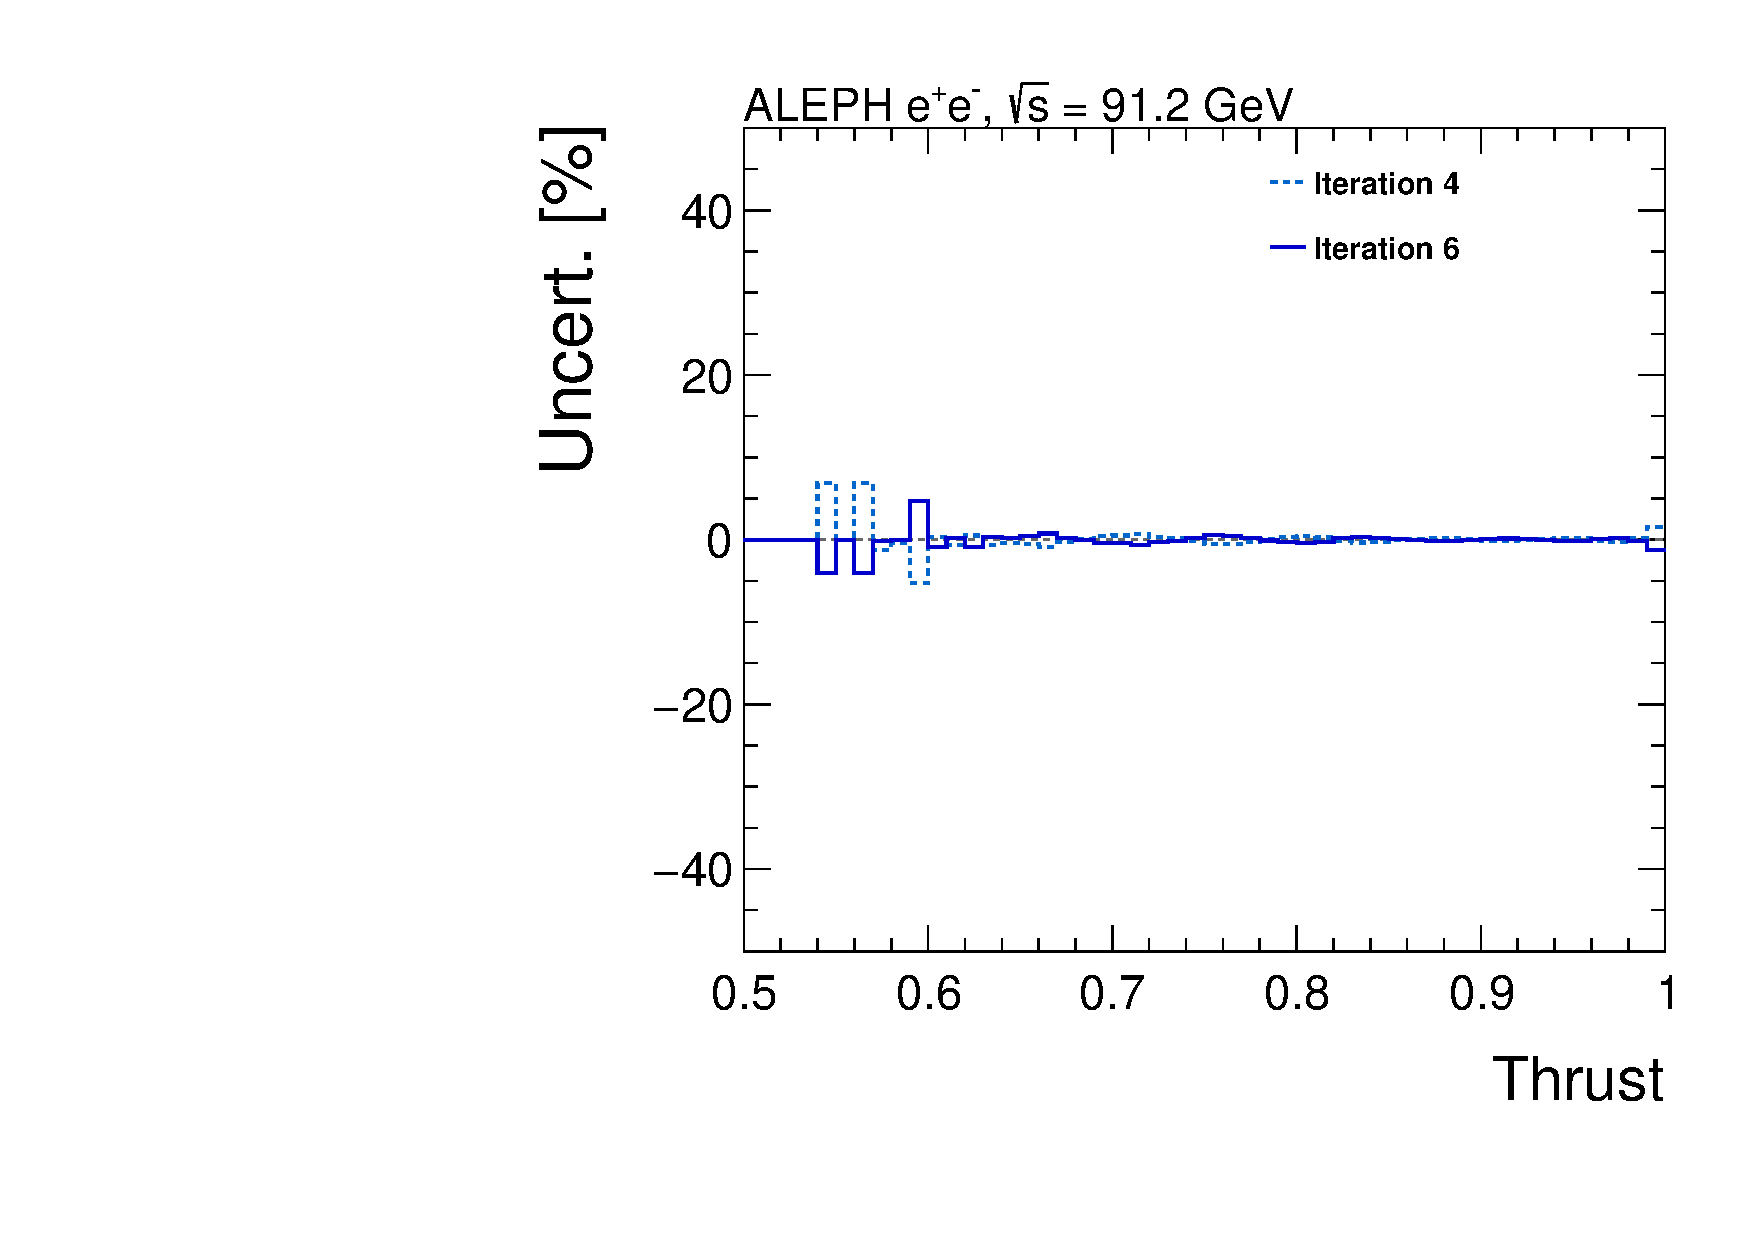
\includegraphics[width=0.49\textwidth]{../Studies/PreliminaryResult/2026-02-17_thrust_iter5/summary/uncertainty_components_unfolding.pdf}
\\
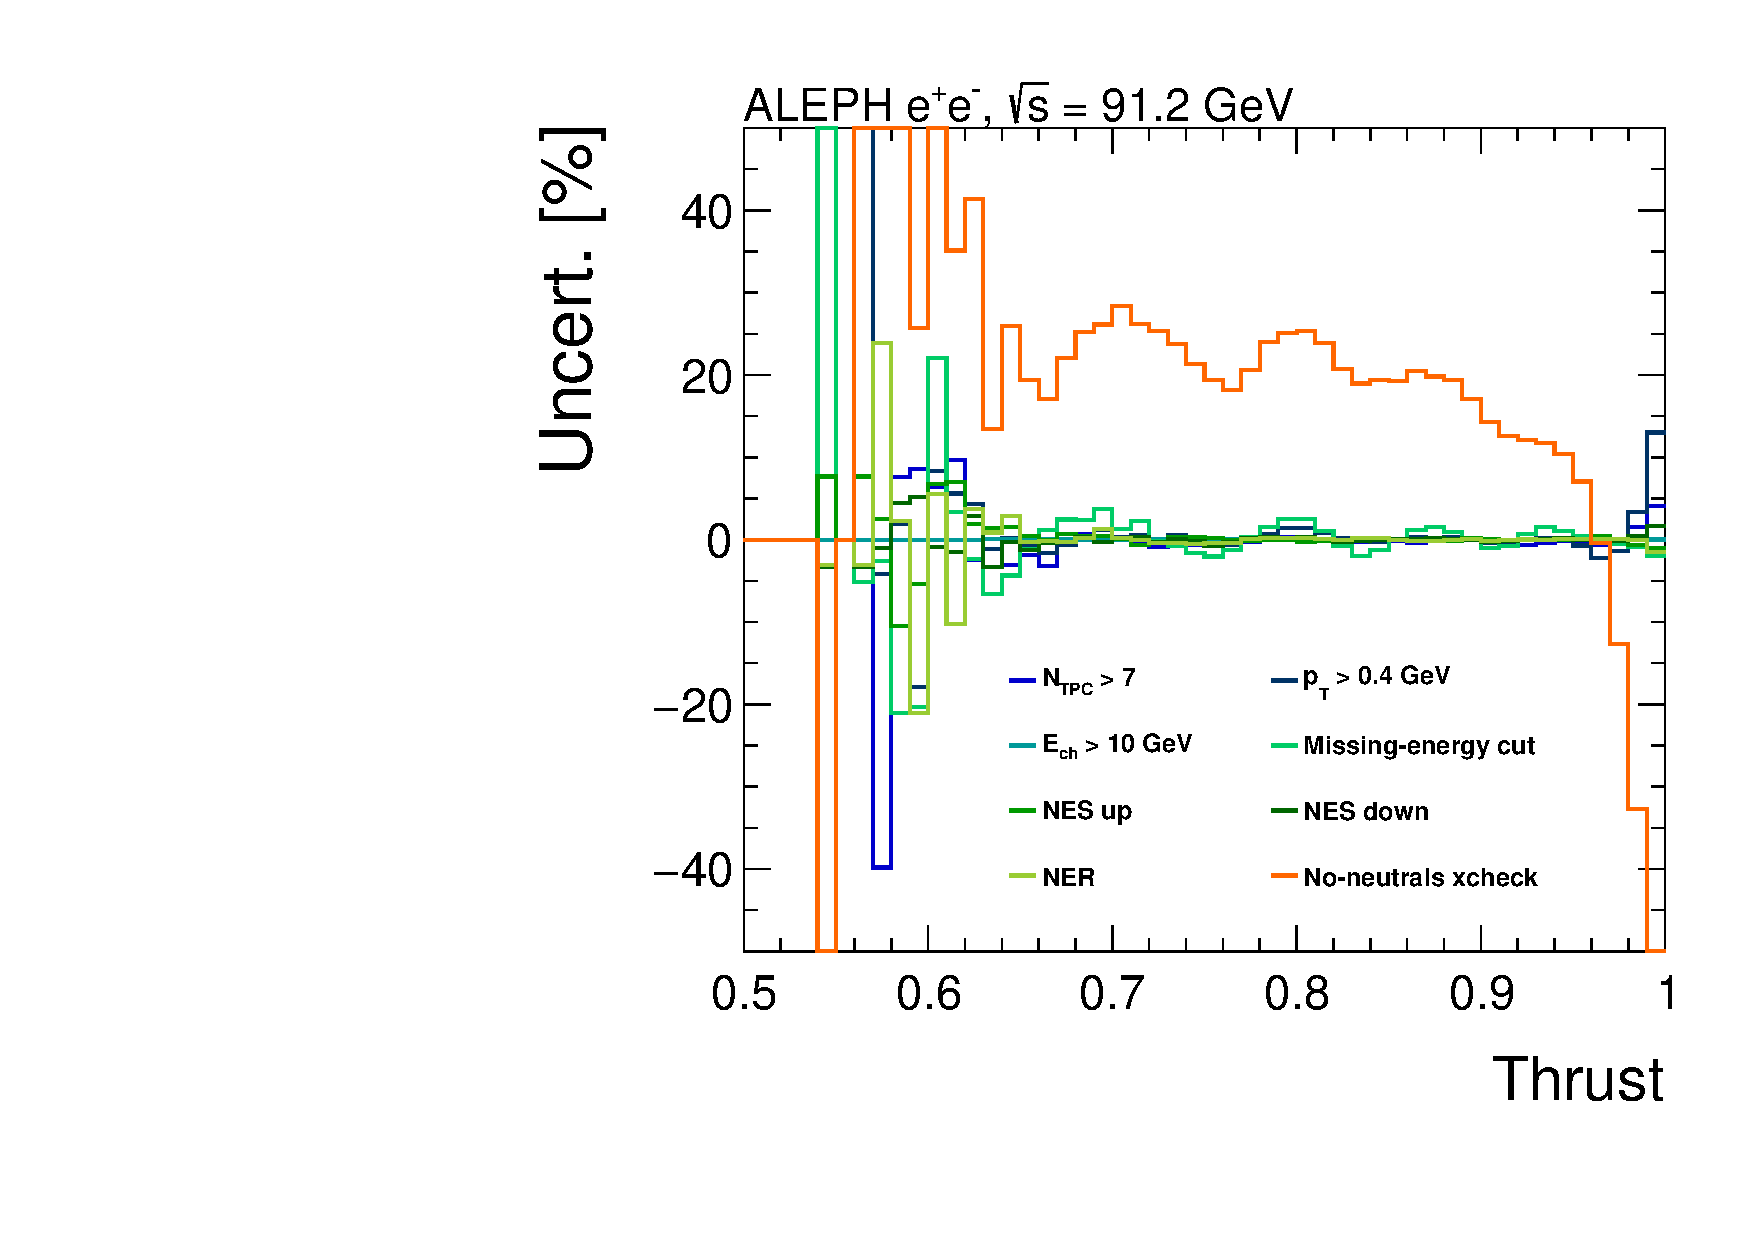
\includegraphics[width=0.49\textwidth]{../Studies/PreliminaryResult/2026-02-17_thrust_iter5/summary/uncertainty_components_experimental.pdf}
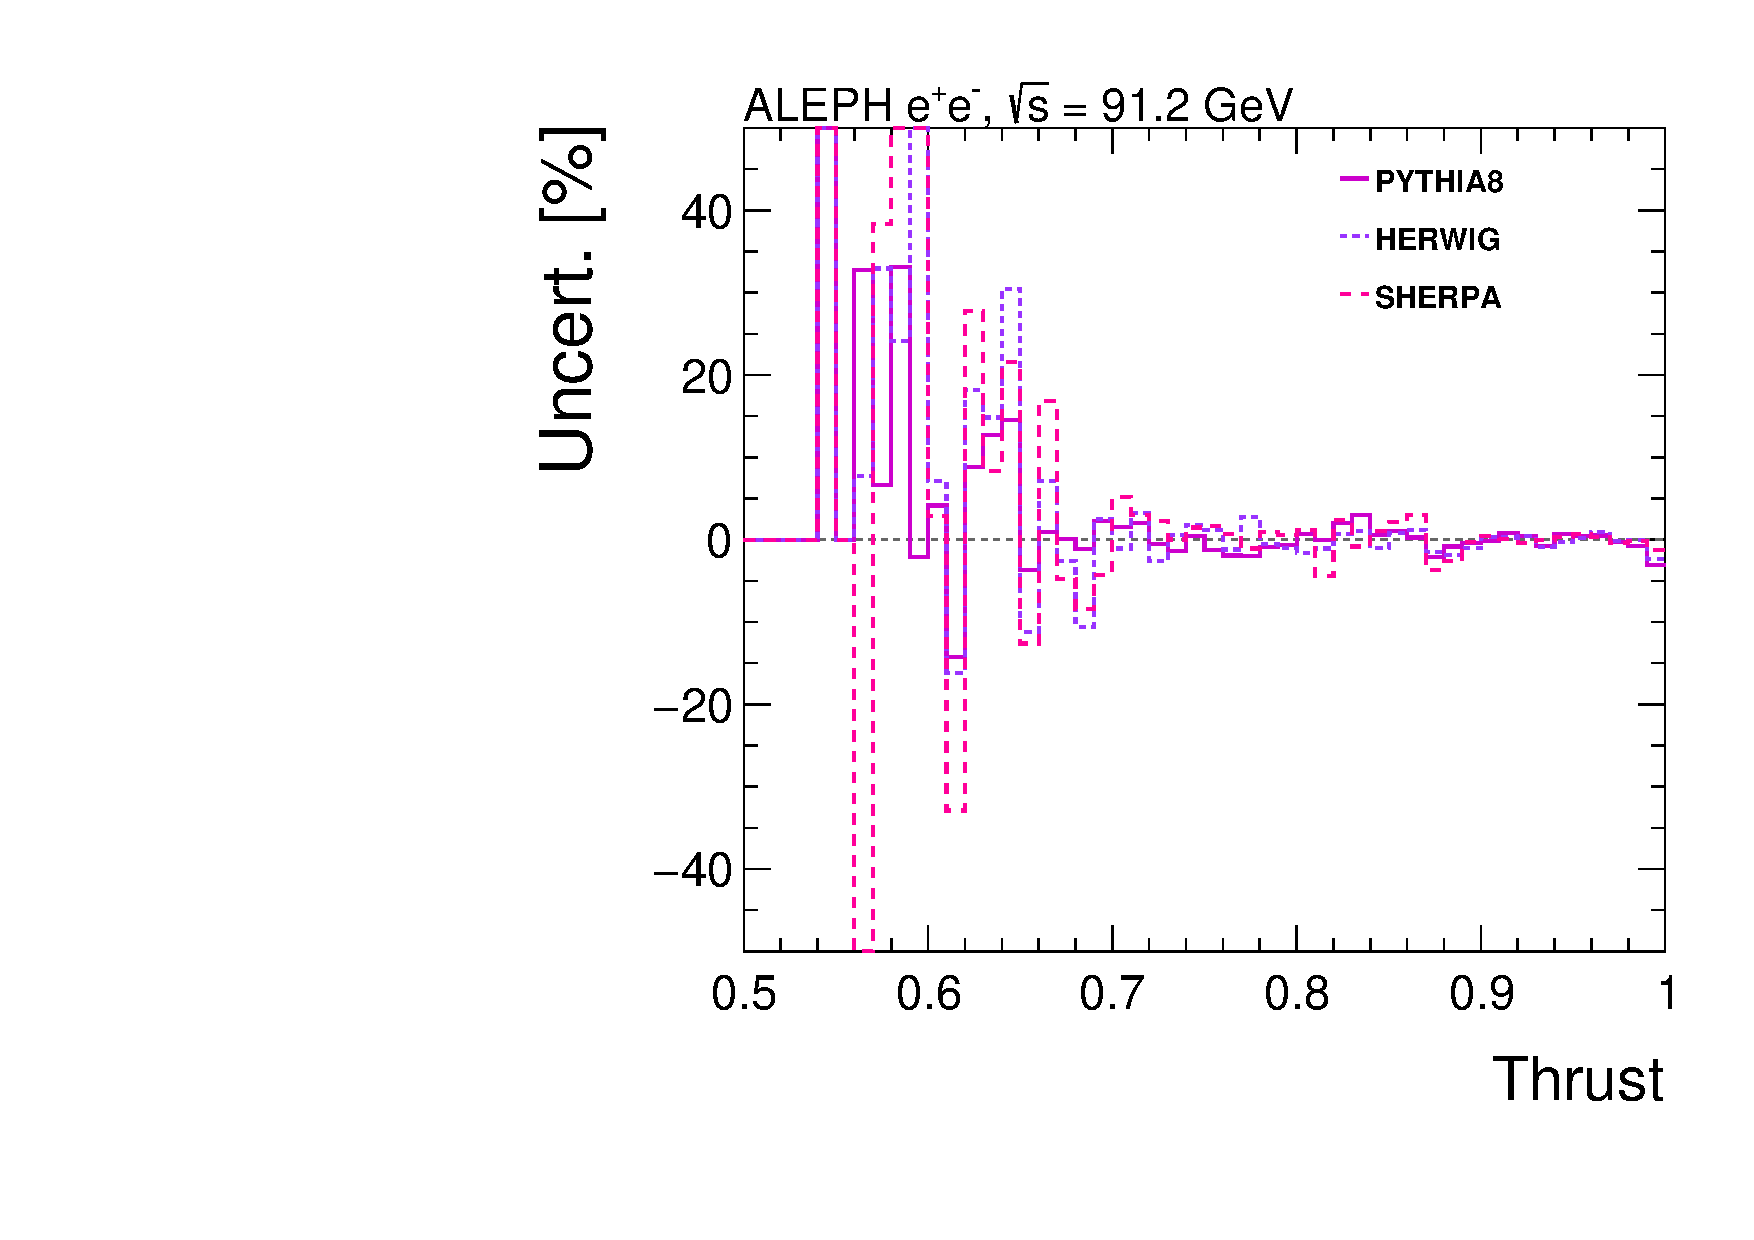
\includegraphics[width=0.49\textwidth]{../Studies/PreliminaryResult/2026-02-17_thrust_iter5/summary/uncertainty_components_theory.pdf}
\caption{Uncertainty components in four views: statistical (top left), unfolding iterations (top right), experimental variations (bottom left), and theory reweighting (bottom right). Non-statistical panels show signed shifts relative to nominal in percent; displayed $y$-ranges are clipped to $\pm 50\%$ for readability.}
\label{fig:uncertainty_components_fourpanel}
\end{figure}

The dominant mean contributions in the central range ($0.60\le T<0.95$) are theory
and experimental components, while the iteration uncertainty is subleading for the
nominal regularization choice. The hadronic correction uncertainty is an additional
independent component. The mean total uncertainty in the central range is $8.43\%$,
dominated by the theory envelope; this figure is derived from the diagonal of the
total covariance matrix in the differential cross-section basis.

\subsection{Final total correlation matrix}

\begin{figure}[t!]
\centering
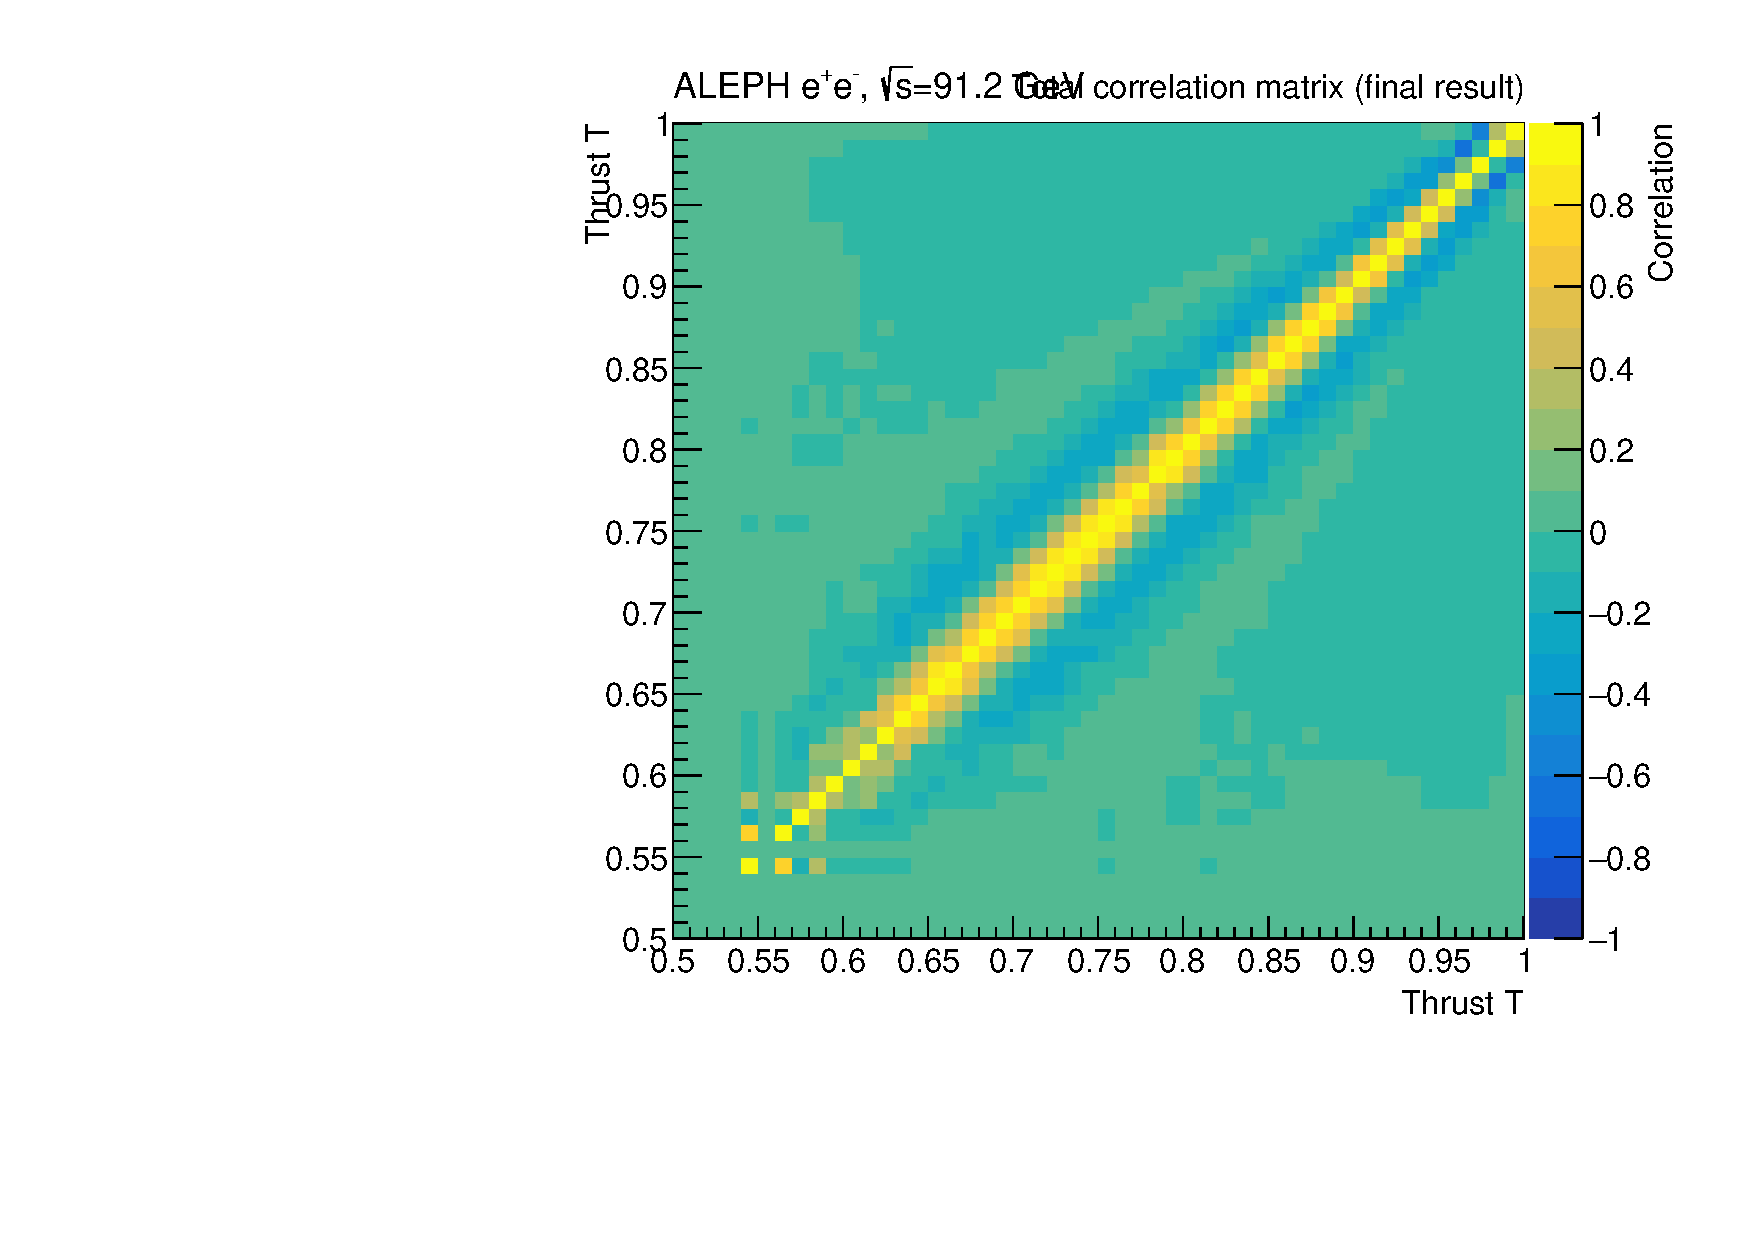
\includegraphics[width=0.82\textwidth]{../Studies/PreliminaryResult/2026-02-17_thrust_iter5/summary/matrix_total_correlation_final.pdf}
\caption{Total bin-to-bin correlation matrix for the final result, combining statistical, unfolding-iteration, experimental, theory, and hadronic-correction components using the \texttt{template\_correlated} covariance model.}
\label{fig:final_total_correlation_matrix}
\end{figure}

Figure~\ref{fig:final_total_correlation_matrix} shows the total correlation structure.
The matrix is non-diagonal, with largest off-diagonal correlation $|\rho_{ij}|=0.889$,
confirming that correlated information is preserved in the exported products intended
for downstream phenomenology.

\subsection{Final unfolded thrust distribution}

\begin{figure}[h!]
\centering
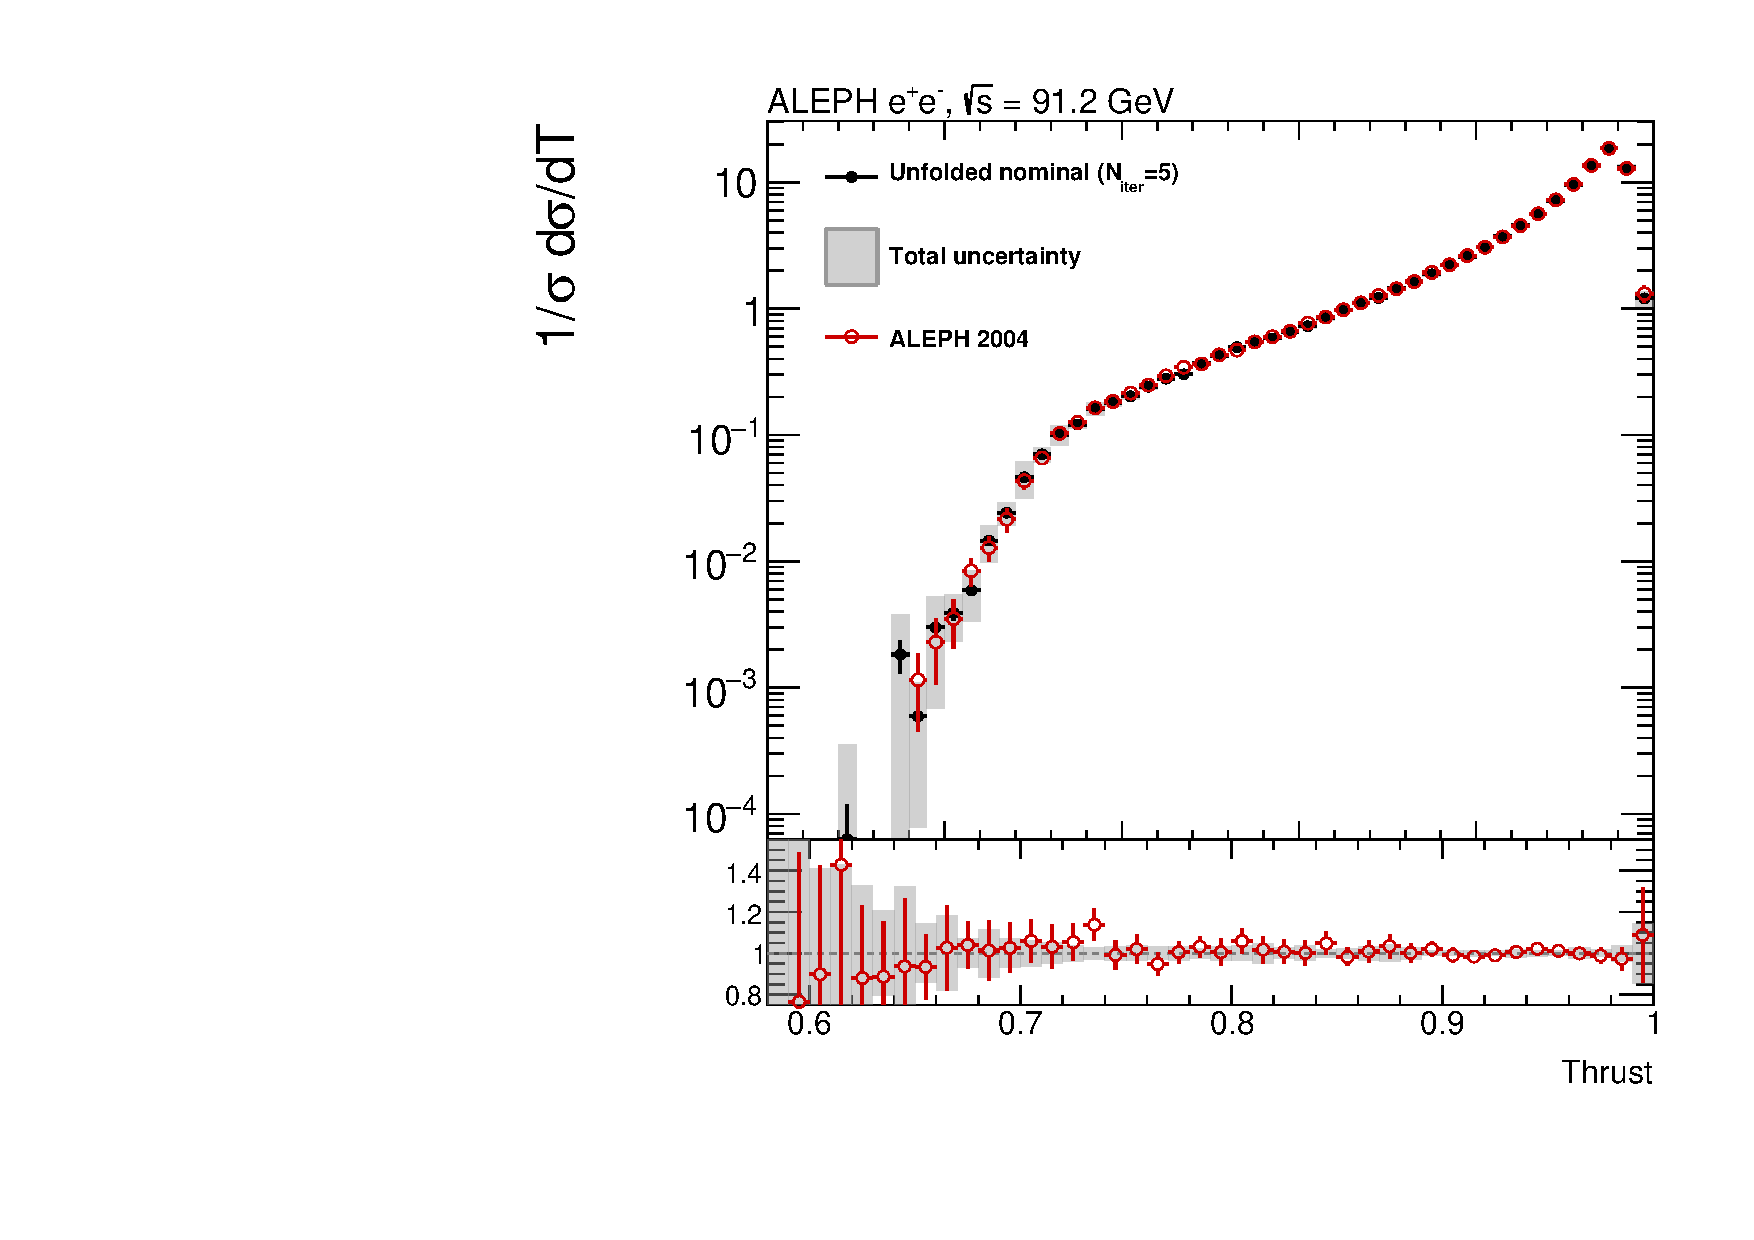
\includegraphics[width=0.48\textwidth]{../Studies/PreliminaryResult/2026-02-17_thrust_iter5/summary/final_result_uncertainty_breakdown.pdf}%
\hfill%
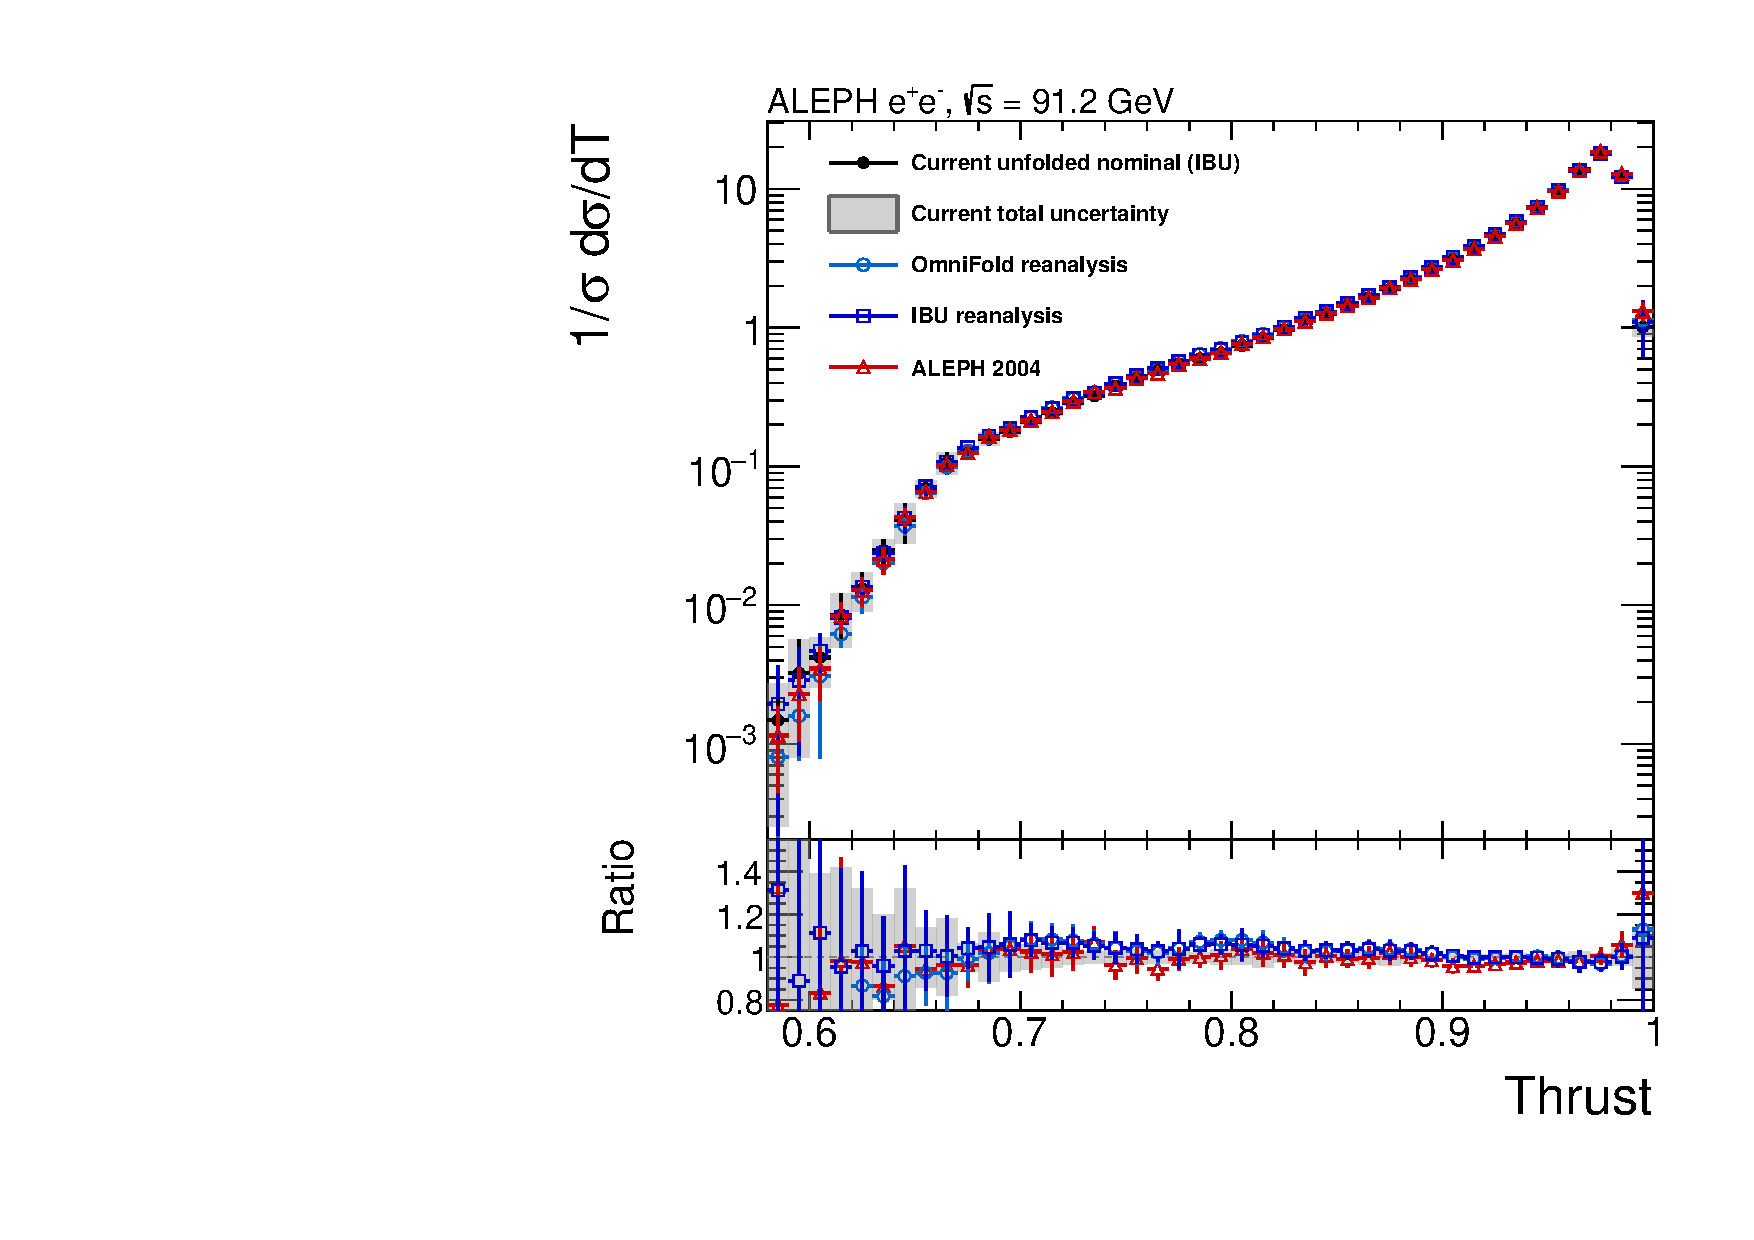
\includegraphics[width=0.48\textwidth]{../Studies/PreliminaryResult/2026-02-17_thrust_iter5/summary/final_result_of_ibu_comparison.pdf}
\caption{Left: final unfolded thrust result with total uncertainty band and comparison to the published ALEPH 2004 result in the ratio panel. Right: comparison with OmniFold and prior IBU reanalyses; the ratio panel shows each curve relative to the current unfolded nominal, with the gray band representing the current total uncertainty.}
\label{fig:final_thrust_result}
\end{figure}

\FloatBarrier

Figure~\ref{fig:final_thrust_result} (left) shows the unfolded spectrum with the total
uncertainty band and comparison to the published ALEPH 2004 result. The largest
discrepancy occurs at the endpoint ($0.99<T<1.00$, ratio $1.30\pm0.27$), which is
physically expected: the dijet limit is sensitive to MC modeling of soft hadrons, the
hadronic correction $C_{\mathrm{had}}(j)$ whose uncertainty grows at the endpoint, and
normalization convention differences between the current analysis and the 2004 ALEPH
publication.

Figure~\ref{fig:final_thrust_result} (right) shows direct comparison with OmniFold and
prior IBU spectra from the archived-data analysis program. Compatibility metrics are
$\chi^2/\mathrm{ndf}=0.663$ (OmniFold), $0.421$ (prior IBU), and $0.361$ (ALEPH 2004),
evaluated over 42 bins using the diagonal of the total covariance. Sub-unity values
reflect the conservative uncertainty model and positive off-diagonal correlations, not
overestimation. Differences are localized to the endpoint region; the diagnostic
program for this region is documented separately.

\subsection{Energy-flow vs charged-only cross-check}
\label{sec:charged_only_crosscheck}

As a cross-check of the neutral-hadron treatment, the unfolding was repeated with
neutral particles (photons and neutral hadrons, $\mathrm{pwflag}\in\{4,5\}$) removed
from the energy-flow objects, yielding a charged-only thrust distribution.
Figure~\ref{fig:charged_vs_ef} compares the charged-only and energy-flow unfolded
spectra and their bin-by-bin ratio.  Both distributions are normalized to unit
integral per bin width.  The charged-only spectrum is systematically softer than the
energy-flow result at low thrust (high multiplicity), as expected from missing neutral
energy deposits, but the ratio remains within $\pm 20\%$ across the central range,
consistent with the $\sim 30\%$ neutral energy fraction reported in prior ALEPH
publications.  No pathological bin-level disagreement is observed, confirming that the
neutral-hadron cleaning cut (Sec.~\ref{sec:neutral_hadron_cleaning}) does not introduce
a bias in the energy-flow thrust distribution.

\begin{figure}[h!]
\centering
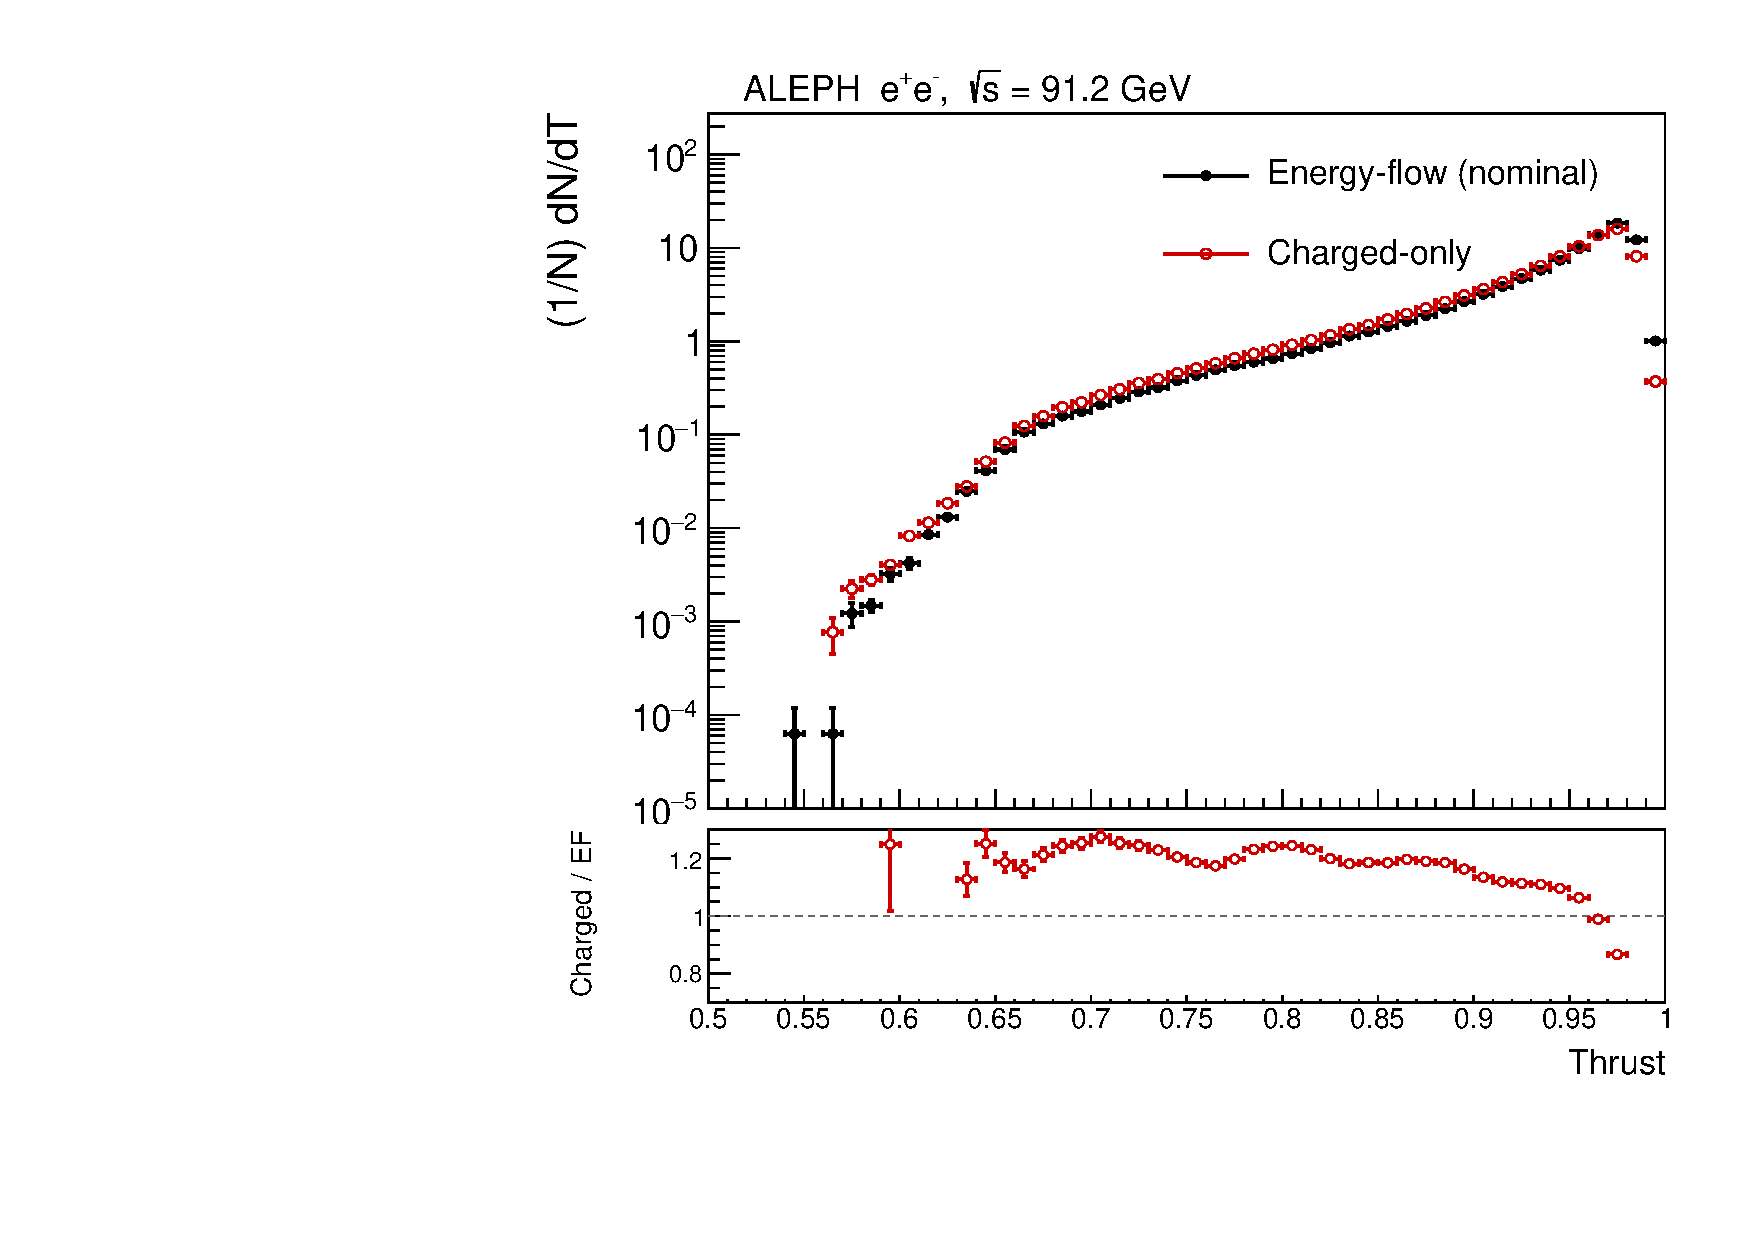
\includegraphics[width=0.70\textwidth]{../Studies/Phase2_Checks_2026-03-03/plots/charged_only_vs_energy_flow/charged_only_vs_energy_flow.pdf}
\caption{Comparison of the charged-only (red open circles) and energy-flow (black filled circles) unfolded thrust distributions, normalized to $(1/N)\,\mathrm{d}N/\mathrm{d}T$.  The ratio panel shows charged-only / energy-flow; the dashed line marks unity.}
\label{fig:charged_vs_ef}
\end{figure}

\FloatBarrier

\subsection{Release products}

The result bundle includes central values, covariance and correlation matrices, binning
definitions, fit-window products, and component-level uncertainty plots. For theory
fits, the recommended inputs are the fit-window covariance products (covering 45 bins
in $0.505\le T < 1.00$) rather than the full-range covariance. All result files are
version-controlled and associated with structured provenance metadata that records the
git commit, software versions, and key analysis parameters used to produce this result.
